\section{Mininet-Wifi CLI}
Es esta sección se va a recorrer todas las funcionalidades que nos ofrece la CLI ( Command Line Interface) de Mininet-Wifi en la medida que sea posible. A continuación, listamos todos los comandos que están disponibles y documentados en la CLI de Mininet-Wifi. \newline
\newline

% Please add the following required packages to your document preamble:
% \usepackage{booktabs}
\begin{table}[!ht]
\centering
\begin{tabular}{|c|c|c|c|c|c|}
\hline
\textbf{EOF}      & \textbf{gterm}    & \textbf{links}   & \textbf{pingallfull}  & \textbf{py}     & \textbf{stop}   \\ \hline
\textbf{distance} & \textbf{help}     & \textbf{net}     & \textbf{pingpair}     & \textbf{quit}   & \textbf{switch} \\ \hline
\textbf{dpctl}    & \textbf{intfs}    & \textbf{nodes}   & \textbf{pingpairfull} & \textbf{sh}     & \textbf{time}   \\ \hline
\textbf{dump}     & \textbf{iperf}    & \textbf{noecho}  & \textbf{ports}        & \textbf{source} & \textbf{x}      \\ \hline
\textbf{exit}     & \textbf{iperfudp} & \textbf{pingall} & \textbf{px}           & \textbf{start}  & \textbf{xterm}  \\ \hline
\end{tabular}
\centering
\end{table}
\subsection{Comando: EOF + quit + exit}
Estos tres comandos se utilizan para lo mismo, salir de la CLI de Mininet-Wifi y terminar la emulación. El código de estos tres comandos no difieren mucho,  son comandos heredados de la CLI de Mininet. EOF y quit terminan haciendo uso de exit al final, por lo que podríamos decir que son un poco repetitivos.
\begin{minted}[]{python}
    def do_exit( self, _line ):
        "Exit"
        assert self  # satisfy pylint and allow override
        return 'exited by user command'

    def do_quit( self, line ):
        "Exit"
        return self.do_exit( line )

    def do_EOF( self, line ):
        "Exit"
        output( '\n' )
        return self.do_exit( line )
\end{minted}
 \subsection{Comando: distance}
 Este comando sirve para medir la distancia entre dos entes de la topología emulada. El uso es muy sencillo, únicamente hay que indicar el nombre dado a cada ente y nos dará la distancia en metros. 
 
 \begin{figure}[!htb]
  \centering
    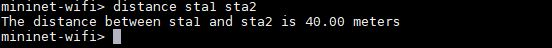
\includegraphics[width=0.8\linewidth]{./img/cli/1.JPG}
    \caption{Comando distance output.}
  \label{fig:yo}
\end{figure}

%% Aquí poner test_topo_1 editada distancia %%

\subsection{Comando: dpctl}
El comando dpctl es un comando heredado de la CLI de Mininet, pero redefinido en el for de Mininet-Wifi con pocas variaciones. Dpctl es un comando de utilidad de administración que permite cierto control sobre el switch OpenFlow (ovs-ofctl en el switch OpenvSwitch). Con este comando es posible agregar flujos a la tabla de flujo, consultar las características y el estado de los switchs y cambiar otras configuraciones, limpiar la tabla entre otras cosas. \newline
\newline
Como se ha dicho este comando tiene bastantes funcionalidades, por no entrar una a una se deja aquí donde se debe ir a consultar cada funcionalidad del comando en función del tipo de switch.
\begin{itemize}
    \item Ofssoftswitch: \url{https://github.com/CPqD/ofsoftswitch13/wiki/Dpctl-Documentation}
    \item OpenvSwitch: \url{http://www.openvswitch.org/support/dist-docs/ovs-ofctl.8.txt}
\end{itemize}
Por lo que se ha podido apreciar en el código del comando, la instrucción se replicará en todos los switches de la topología.
\begin{minted}[]{python}
def do_dpctl(self, line):
        """Run dpctl (or ovs-ofctl) command on all switches.
           Usage: dpctl command [arg1] [arg2] ..."""
        args = line.split()
        if len(args) < 1:
            error('usage: dpctl command [arg1] [arg2] ...\n')
            return
        nodesL2 = self.mn.switches + self.mn.aps
        for sw in nodesL2:
            output('*** ' + sw.name + ' ' + ('-' * 72) + '\n')
            output(sw.dpctl(*args))
            
#Nota: Nosotros utilizaremos sobretodo dpctl dump-flows y 
# dpctl del-flows para consultar o limpiar las tablas de flujo.
\end{minted}

\subsection{Comando: dump + net}
Estos comandos nos arrojarán información sobre la topología emulada. El comando net nos indicará los nombres de los entes que hay en la topología a emular y sus interfaces. El comando dump además nos indicará el tipo de ente, dirección IP, puerto cuando corresponda, interfaz y el identificador de proceso (pid) del ente.

 \begin{figure}[!htb]
  \centering
    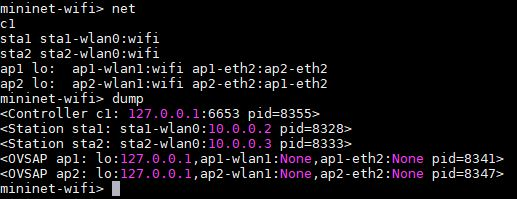
\includegraphics[width=0.8\linewidth]{./img/cli/2.JPG}
    \caption{Comando net y dump output.}
  \label{fig:yo}
\end{figure}
\subsection{Comando: xterm y gterm}
Estos dos comandos nos permitirán abrir terminales en el nodo indicado. El comando \textbf{xterm} nos permitirá abrir una terminal simple, y el comando \textbf{gterm} nos permitirá abrir una gnome-terminal. Podemos abrir varias terminales a la vez indicando todos los nodos que queremos abrir una terminal en ellos.\newline Uso xterm/gterm [node1] [node2] ... \newline
\newline
 \begin{figure}[!htb]
  \centering
    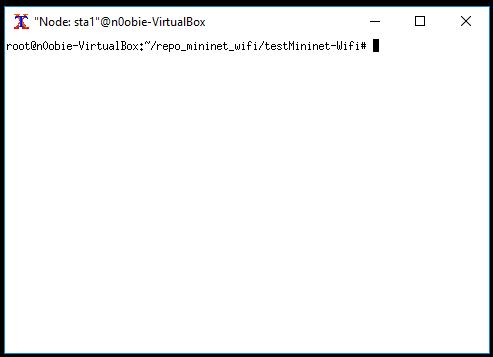
\includegraphics[width=0.8\linewidth]{./img/cli/3.JPG}
    \caption{Ejemplo comando xterm.}
  \label{fig:yo}
\end{figure}
 \begin{figure}[!htb]
  \centering
    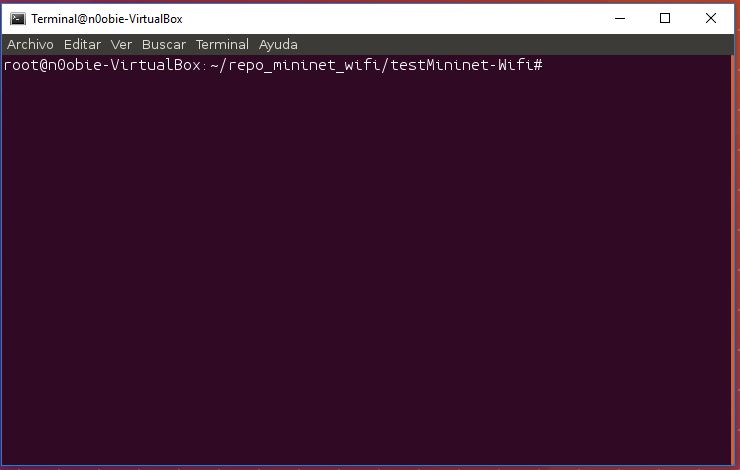
\includegraphics[width=0.7\linewidth]{./img/cli/4.JPG}
    \caption{Ejemplo comando gterm.}
  \label{fig:yo}
\end{figure}
\subsection{Comando: help}
El comando por excelencia para visualizar las indicaciones o posible ayuda sobre la operativa de funcionamiento de un programa o comando. Es un comando heredado desde Mininet, al que Mininet-Wifi ha añadido sus nuevas características. Podemos hacer uso de él únicamente escribiendo \textbf{help}. Además podemos obtener información extra de otros comandos utilizando \textbf{help comando}.
\subsection{Comando: intfs + nodes + ports}
Estos comandos listarán información relativa a los nodos de la topología. El comando \textbf{intfs} listará toda la información relativa a las interfaces de los nodos. El comando \textbf{nodes} listará todos los nodos de la topología y el comando, \textbf{ports} utilizado más bien en Mininet se utilizaba para listar los puertos e interfaces de los switches  de la topología. 
 \begin{figure}[!htb]
  \centering
    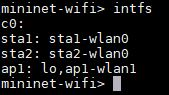
\includegraphics[width=0.4\linewidth]{./img/cli/5.JPG}
    \caption{Ejemplo comando intfs.}
  \label{fig:yo}
\end{figure}
 \begin{figure}[!htb]
  \centering
    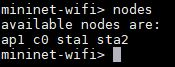
\includegraphics[width=0.4\linewidth]{./img/cli/6.JPG}
    \caption{Ejemplo comando nodes.}
  \label{fig:yo}
\end{figure}
\subsection{Comando: iperf + iperfudp}
Estos comandos nos ayudarán a hacer un benchmark de las capacidades de la topología. Podemos indicar la parte cliente y al parte servidor o dejar a elección de Mininet-Wifi la decisión de entre que extremos hacer el test de iperf. La única diferencia entre el comando \textbf{iperf} y \textbf{iperfudp} es que uno emplea tráfico TCP para hacer el test y el otro hace uso de tráfico UDP para hacer el test. Una vez completado el test podremos apreciar el resultado en Mbits/s. Para más información sobre la herramienta \textbf{iperf} consulte el punto \textbf{A de los anexos}. \newline
\newline
 \begin{figure}[!htb]
  \centering
    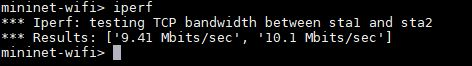
\includegraphics[width=0.7\linewidth]{./img/cli/7_a.JPG}
    \caption{Ejemplo de benchmark con Iperf.}
  \label{fig:yo}
\end{figure}
\newpage
\subsection{Comando: links}
Este comando nos arrojará información sobre el estado de los enlaces de la topología. Este comando, aunque ha sido heredado de Mininet, éste ha sido adaptado a los nuevos enlaces de características Wireless de Mininet-Wifi. \newline
\newline
 \begin{figure}[!htb]
  \centering
    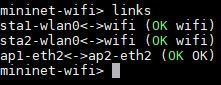
\includegraphics[width=0.4\linewidth]{./img/cli/7.JPG}
    \caption{Ejemplo comando links.}
  \label{fig:yo}
\end{figure}
\subsection{Comando: noecho}
Comando completamente heredado de Mininet. Su funcionalidad reside en ejecutar un comando en uno de los nodos de forma silenciosa, sin sacar por pantalla ningún tipo de información sobre el comando. Para hacer test de este comando y comprender bien bien la salida estándar se ha leído este articulo, muy interesante para entender el concepto de tty y sus opciones: \url{http://www.linusakesson.net/programming/tty/index.php} \newline
\begin{minted}[]{python}
    def do_noecho( self, line ):
        """Run an interactive command with echoing turned off.
           Usage: noecho [cmd args]"""
        if self.isatty():
            # Modo silencioso
            quietRun( 'stty -echo' )
            
        self.default( line )
        
        if self.isatty():
            # Lo volvemos a poner de manera estándar
            quietRun( 'stty echo' )
\end{minted}
\subsection{Comando: pingall + pingallfull}
Estos comandos nos permitirán hacer ping entre todos los host y las estaciones wifi. Por lo que se ha estado testeado pingall funciona según la descripción de su uso. Por el contrario el comando pingallFull no funcionaba, se ha estado investigando y depurando el código, y hemos llegado a la conclusión de que el código estaba obsoleto, ya que al ser un fork de Mininet únicamente incluía a Host con una interfaz alámbrica y no a las estaciones Wifi. Por lo que se ha modificado el código en un fork de Mininet-Wifi para así dotar de la funcionalidad que supuestamente debía tener. Acto seguido se ha abierto otro pull-request para añadir esta modificación en el master de Mininet-Wifi, aquí pueden comprobar el seguimiento de esta modificación.\newline
\newline
\begin{center}
    \url{https://github.com/intrig-unicamp/mininet-wifi/pull/230}
\end{center}
\newpage
\begin{figure}[!htb]
  \centering
    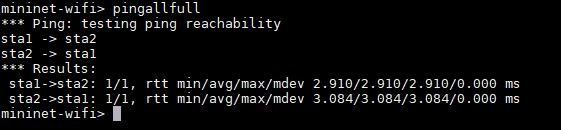
\includegraphics[width=0.7\linewidth]{./img/cli/pullrequest_2.JPG}
    \caption{Posible futuro funcionamiento del comando pingallfull.}
  \label{fig:yo}
\end{figure}
\subsection{Comando: pingpair + pingpairfull}
Los comandos \textbf{pingpair} y \textbf{pingpairfull} son análogos a los expuestos anteriormente. La diferencia reside en el hecho de que ya no es un ping entre todos los host y estaciones Wifi, si no, por parejas. 

\subsection{Comando: px + py}
Estos comandos pueden ser similares, pero la diferencia reside en el hecho de que el comando px ejecuta código python y el comando py evalúa una sentencia de código python. Pero, ¿Cual es la diferencia entre evaluar y ejecutar? Hay dos diferencias importantes:
\begin{itemize}
    \item La primera de ellas, es que a la hora de evaluar, evaluamos un única expresión. Mientras que si hablamos de ejecución podemos ejecutar un bloque entero de código (Una función entera, un bloque try/catch, una clase). Ojito! O.o una declaración no es una expresión.
    \item La segunda diferencia reside en el hecho de que una evaluación de código siempre retorna el valor/resultado de la expresión dada. Por el contrario la ejecución ignora el valor/resultado de una expresión deberemos obligarle a retornarlo por ejemplo haciendo print de la expresión a ejecutar.  
\end{itemize}
Expuesto esta diferencias se debería entender el resultado y la forma en la que se han ejecutado ambos comandos para obtener el mismo resultado.\newline
\newline
\begin{figure}[!htb]
  \centering
    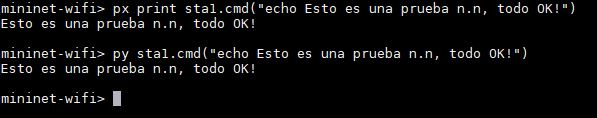
\includegraphics[width=\linewidth]{./img/cli/8.JPG}
    \caption{Ejemplo funcionamiento comandos px y py.}
  \label{fig:yo}
\end{figure}
\subsection{Comando: sh}
Este comando tiene una gran importancia ya que es nuestra puerta a ejecutar código fuera de la CLI de Mininet-Wifi. El output de dicho comando es redirigido a la CLI de Mininet-Wifi, su uso es muy sencillo únicamente hay que poner el comando sh y el comando a ejecutar. Ejemplo: \textbf{sh ifconfig}.
\begin{figure}[!htb]
  \centering
    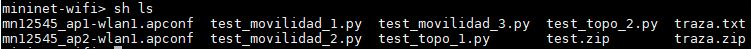
\includegraphics[width=\linewidth]{./img/cli/9.JPG}
    \caption{Ejemplo funcionamiento comando sh.}
  \label{fig:yo}
\end{figure}
\newpage
\subsection{Comando: source}
El comando source tiene como funcionalidad de ejecutar un fichero con comandos de la CLI de Mininet-Wifi. Por así decirlo es un comando que nos permite lanzar Mininet-Wifi CLI scripts (Podríamos llamar a los ficheros con ordenes por ejemplo \textbf{MWCLI-scripts}). Puede que esto se vea un poco abstracto por lo que vamos a poner ejemplo de uso. En un fichero llamado por nosotros comando.txt vamos a introducir linea a linea comandos que queremos ejecutar en la CLI de Mininet-Wifi. Esto nos ahorrará el tiempo de escribirlos cuando lancemos la CLI de Mininet-Wifi  y agotaremos menos tiempo de la emulación.\newline
\begin{figure}[!htb]
  \centering
    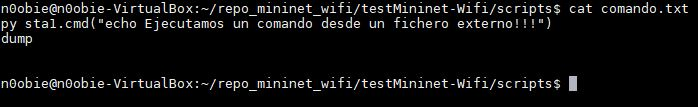
\includegraphics[width=\linewidth]{./img/cli/10.JPG}
    \caption{Contenido del fichero comandos.txt.}
  \label{fig:yo}
\end{figure}
\newline
Una vez dentro de CLI de Mininet-Wifi podemos llamar a nuestro MWCLI script con el comando source, el resultado es el siguiente. (El echo sale corrupto aun no sé a ciencia cierta el por qué, pero sospecho que se debe a que había un mensaje en sta1 en cola para ser dirigido por la salida estándar y a salido con nuestra orden de echo).
\begin{figure}[!htb]
  \centering
    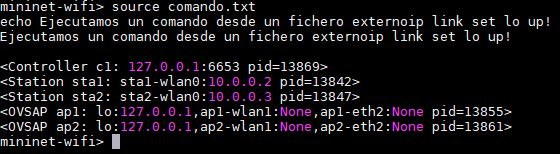
\includegraphics[width=\linewidth]{./img/cli/11.JPG}
    \caption{Ejemplo funcionamiento comando source.}
  \label{fig:yo}
\end{figure}
\subsection{Comando: start + stop}
En teoría estos comandos, añadidos en Mininet-Wifi tienen como funcionalidad la de  parar/iniciar la movilidad en los nodos de la topología. No funciona. Se ha hecho debug y se ha visto que lo único que hacen es modificar una variable booleana llamada
pause\_simulation pero no hacen nada con ella después. Si tengo tiempo arreglaré esto y presentaré el tercer pull-request para que lo añadan al master.
\begin{minted}[]{python}
# cli.py

def do_stop(self, line):
        "stop mobility for a while"
        self.mn.stop_simulation()

def do_start(self, line):
        "pause mobility for a while"
        self.mn.start_simulation()
        
\end{minted}
\newpage
\begin{minted}[]{python}
# net.py clase Mininet_Wifi (obj mn)

    @staticmethod
    def stop_simulation():
        "Pause the simulation"
        mob.pause_simulation = True

    @staticmethod
    def start_simulation():
        "Start the simulation"
        mob.pause_simulation = False
        
\end{minted}
\begin{minted}[]{python}
# mobility.py

class mobility(object):
...
pause_simulation = False
...
\end{minted}
\subsection{Comando: switch}
El comando switch es un comando heredado de la CLI de Mininet. Su funcionalidad era la de parar o reanudar un switch dado el nombre y la operación de start/stop. Sintaxis:\newline
\begin{minted}[]{python}
switch <switch name> {start,stop}
\end{minted}
\subsection{Comando: time}
El comando time es similar al comando time de la terminal de Linux. Se utiliza para sacar el tiempo que se consume en ejecutar una orden dada.  
\begin{figure}[!htb]
  \centering
    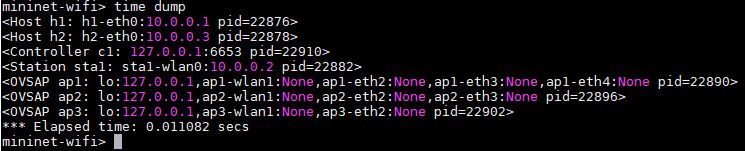
\includegraphics[width=\linewidth]{./img/cli/12.JPG}
    \caption{Ejemplo funcionamiento comando time.}
  \label{fig:yo}
\end{figure}
\subsection{Comando: x}
El comando \textbf{x} se utiliza para crear un canal x11 a un nodo dado. Es muy útil para abrir aplicaciones con una interfaz gráfica. Ejemplo:
\begin{figure}[!htb]
  \centering
    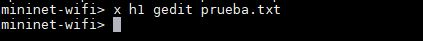
\includegraphics[width=0.7\linewidth]{./img/cli/13.JPG}
    \caption{Ejemplo funcionamiento comando x.}
  \label{fig:yo}
\end{figure}
\newpage
\begin{figure}[!htb]
  \centering
    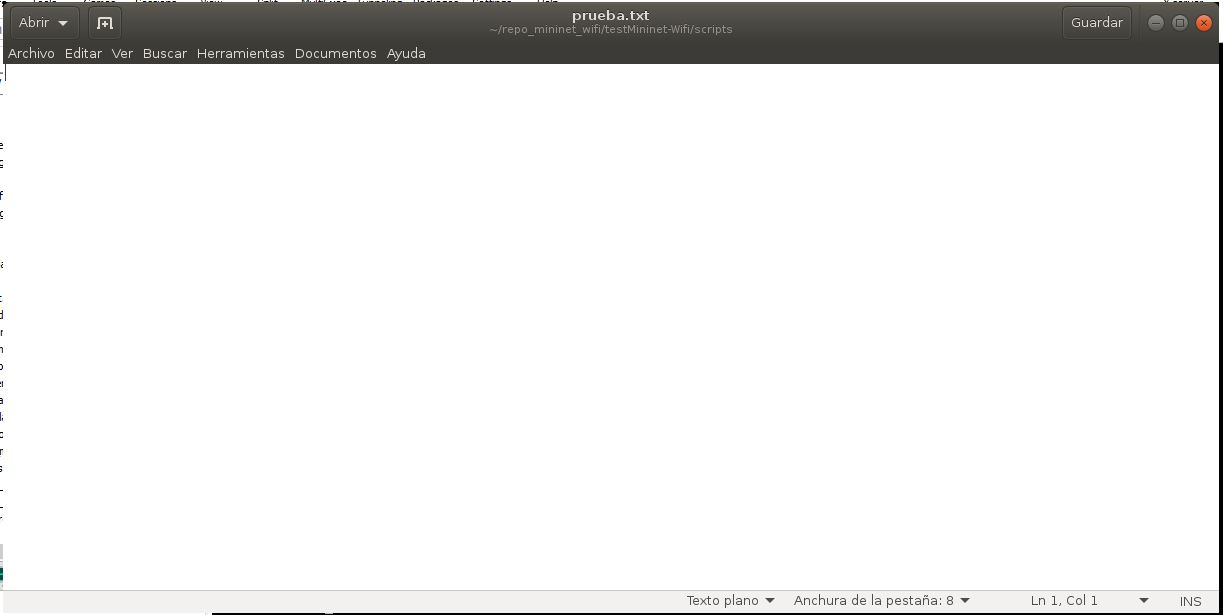
\includegraphics[width=\linewidth]{./img/cli/14.JPG}
    \caption{GUI de gedit en el Host 1.}
  \label{fig:yo}
\end{figure}
